\setchapterpreamble{
    \lettrine{N}{o}~theory is worth its salt without experiments to put it to the test~\cite{Popper:1959}.
    This thesis, in particular, focuses on the flavour physics section of the SM.
    The measurements used to test this part of the theory are performed using the Large Hadron Collider at \cern~(\cref{sec:LHC}) and the \lhcb~experiment in particular~(\cref{sec:LHCb}).}
\chapter{The \lhc and the \lhcb experiment}
\label{chp:detector}

\vspace*{\fill}
\minitoc

\clearpage
\section{The \lhc}
\label{sec:LHC}

The Large Hadron Collider~(\lhc)~\cite{Evans:1129806} is a \SI{27}{\km}~long underground particle accelerator located near Geneva, Switzerland.
It is designed to collide two beams of protons with a centre-of-mass energy of up to~\SI{13}{\TeV}, or heavy ions with an energy of up to a few~\si{\TeV} per nucleon.
In~2010, it started operations, and it has been running successfully since.

Before particles are injected into the~\lhc, they are preaccelerated by several other accelerators, as can been seen in \cref{fig:detector_LHC}.
Protons start in Linac~2, where they are accelerated up to~\SI{50}{\MeV}.
They are subsequently injected into the Proton Synchrotron Booster~(\SI{1.4}{\GeV}), Proton Synchrotron (PS,~\SI{25}{\GeV}), and Super Proton Synchrotron (\sps,~\SI{450}{\GeV}).
From the~\sps, they are then injected into the~\lhc.
When completely filled, each of the two beams in the~\lhc contain \num{2808}~bunches of about \num{e11}~protons each, guided along the circular trajectory by superconducting magnets, cooled to~\SI{1.9}{\kelvin}.
The beams are made to collide at four points along the accelerator: at the \atlas~detector, the \alice~detector, the \cms~detector, and the \lhcb~detector.
This thesis focuses on the last.
%
\begin{figure}[htb] \centerfloat
    \hspace*{-.5cm}
    \includegraphics[width=1.1\textwidth]{detector/cern-accelerators}
    \caption{
        The \cern~accelerator complex, including the~\lhc, its preaccelerators, and its four largest detectors.
        Various other experiments are also shown.
        Image adapted from Ref.~\cite{Mobs:2197559}.}
    \label{fig:detector_LHC}
\end{figure}

\clearpage
\section{The \lhcb experiment}
\label{sec:LHCb}

The \lhcb~detector (\cref{fig:detector_LHCb})~\cite{1748-0221-3-08-S08005,LHCb-DP-2014-002} consists of various subdetectors, each providing different particle detection capabilities.
The detector is unique at the~\lhc for operating only in the forward direction, that is, it only detects particles with a pseudorapidity between~\num{2} and~\num{5}.
Central to the setup is a dipole magnet, providing a magnetic field with a bending power of~\SI[inter-unit-product=]{4}{\tesla\metre} to bend the particles' trajectories and enable measurements of their momenta.
Several subdetectors, both upstream (before, from the point of view of a particle emanating from a \({\proton\proton}\)~collision) and downstream (after) the magnet, are specifically engineered such that their combined measurements result in an accurate reconstruction of the collision and the resulting decay products.
%
\begin{figure}[htb] \centerfloat
    \hspace*{-.5cm}
    \begin{tikzpicture}[font=\captionfont]
        \node[anchor=south west,inner sep=0] (image) at (0,0) {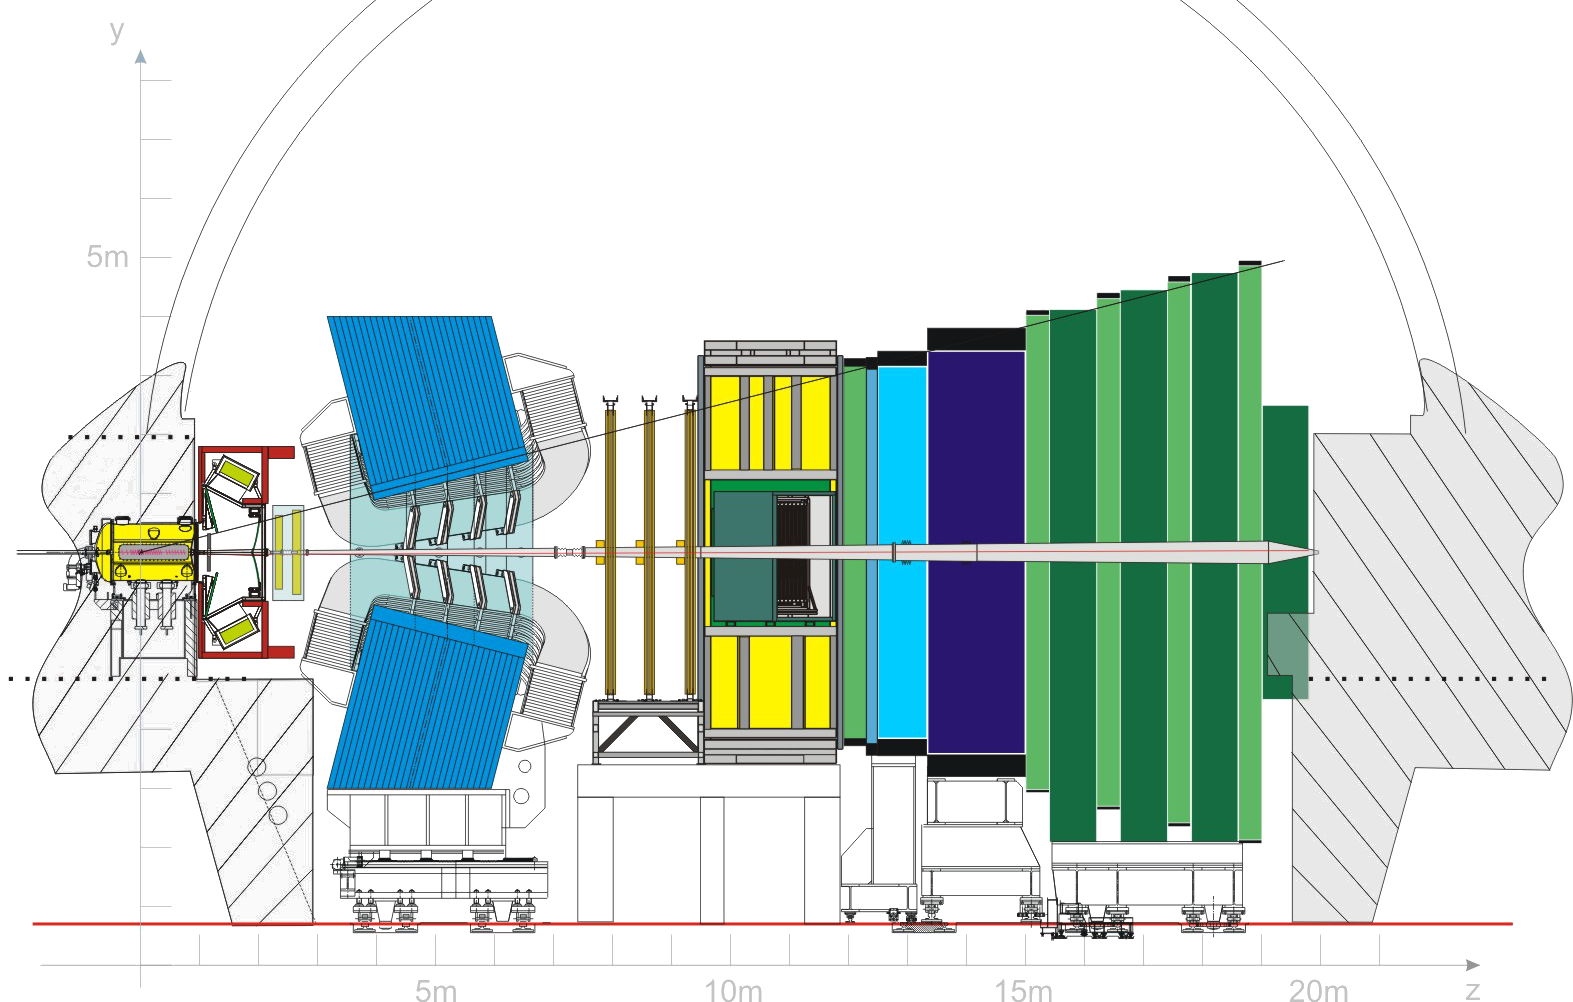
\includegraphics[width=1.\textwidth]{detector/LHCb}};
        \begin{scope}[x={(image.south east)},y={(image.north west)}]
            \draw [very thick, ->] (-.1, .45) -- (.01, .45) node [at start,anchor=north west] {\normalsize \proton};
            \draw [very thick, ->] (.95, .45) -- (.84, .45) node [at start,anchor=north east] {\normalsize \proton};

            \draw [very thick] (.11, .47) -- (.11, 0.85) node [right,anchor=north west,inner ysep=0pt,outer sep=0pt] {\velo};
            \draw [very thick] (.16, .54) -- (.16, 0.80) node [right,anchor=north west,inner ysep=0pt,outer sep=0pt] {\rich~1};
            \draw [very thick] (.185,.48) -- (.185,0.75) node [right,anchor=north west,inner ysep=0pt,outer sep=0pt] {\ttracker};
            \draw [very thick] (.27, .65) -- (.27, 0.85) node [right,anchor=north west,inner ysep=0pt,outer sep=0pt] {Magnet};
            \draw [very thick] (.413,.57) -- (.413,0.85) node [right,anchor=north west,inner ysep=0pt,outer sep=0pt] {\intr~\&~\ot};
            \draw [very thick] (.46, .61) -- (.46, 0.78) node [right,anchor=north west,inner ysep=0pt,outer sep=0pt] {\rich~2};
            \draw [very thick] (.57, .61) -- (.57, 0.85) node [right,anchor=north west,inner ysep=0pt,outer sep=0pt] {\presh~\&~\ecal};
            \draw [very thick] (.62, .63) -- (.62, 0.78) node [right,anchor=north west,inner ysep=0pt,outer sep=0pt] {\hcal};
            \draw [very thick] (.75, .67) -- (.75, 0.85) node [right,anchor=north west,inner ysep=0pt,outer sep=0pt,align=left] {Muon\\stations};
        \end{scope}
    \end{tikzpicture}
    \caption{
        Cutout of the \lhcb~detector, with the magnet and the various subdetectors indicated.
        The \({\proton\proton}\)~collisions occur on the left side of the figure, inside the~\velo.}
    \label{fig:detector_LHCb}
\end{figure}

\subsection{Tracking and vertexing}
\label{sec:tracking}

Tracking in the \lhcb~detector is performed by four subdetectors: the Vertex~Locator (\velo) and the double-layered~\ttracker upstream of the magnet, three stations of Inner and Outer Trackers (\intr and \ot), and five Muon stations downstream of the magnet.

The \velo~\cite{LHCb-DP-2014-001} consists of \num{42}~modules of silicon strip detectors centred around the beam pipe, with strips oriented in the radial and angular directions.
The silicon is cooled to an operational temperature of~\SI{-7}{\degreeCelsius}, and a motion system can move the modules closer to the beam pipe after the proton beams in the~\lhc have been focused, until the modules arrive at a distance of~\SI{8}{\mm} from the beam pipe.
The modules are semi-circular, and are placed in pairs of R-sensors (radial strips) and \(\phi\)-sensors (circular strips), which together allow for three-dimensional track reconstruction.
This setup gives a vertex resolution of~\SI{71}{\micro\meter} along the beam axis and \SI{13}{\micro\meter}~in the transverse plane.

The \ttracker~\cite{Gassner:728548} and \intr~\cite{LHCb-TDR-008} also both employ silicon strips to detect particles.
The~\ttracker is located upstream of the magnet, and consists of two stations.
The \intr~has three stations, and is located downstream of the magnet, close to the \lhc~beam pipe.
Each station contains four detection layers, of which the outer two are oriented vertically, and the inner two at a \(\pm\ang{5}\)~stereo angle.
These trackers each have a hit resolution of about~\SI{50}{\micro\meter}.
The \ot~\cite{LHCb-DP-2013-003} surrounds the \intr, and is made up of three stations of gas detectors.
Again, each station consists of four planes of straw tube modules, oriented the same way as in the~\ttracker and~\intr.
The \ot has a hit resolution of about~\SI{200}{\micro\meter}.
Finally, the muon system~\cite{LHCb-DP-2012-002,LHCb-DP-2013-001} consists of five stations of multi-wire proportional chambers (MWPCs), four of which are located downstream from the calorimeter systems, such that muons can be identified as they traverse the calorimeters, while keeping most of their momentum.
Due to the high particle density in the muon detector upstream of the calorimeter, its inner part is equipped with gas electron multiplier (\gem)~chambers.

Together, the tracking stations allow for the finding and fitting of tracks, the latter of which is done using a Kalman filter approach~\cite{Hulsbergen2005566}.
However, sometimes tracks are reconstructed from hits that do not correspond to the same physical object.
Such a nonphysical track is called a ghost track.
Neural networks are trained to identify them and yield an estimate of the probability of any particular track being a ghost track, allowing rejection of probable ghost tracks.
The most discriminating quantity in determining whether a track is a ghost track is the track~\chisqndf, which is defined as the~\chisq of the track fit divided by the number of degrees of freedom of that fit.
Low values indicate a good track fit, and correspondingly a low probability of that track being a ghost track.

\begin{figure}[htb] \centerfloat
    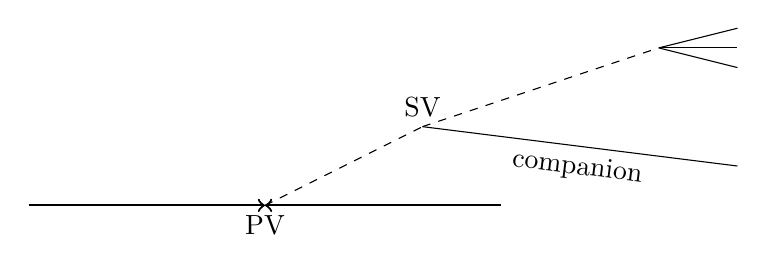
\begin{tikzpicture}[font=\captionfont]
        \coordinate (PV) at (0, 0);
        \coordinate (p1) at (-3, 0);
        \coordinate (p2) at (3, 0);
        \coordinate (Bs) at (2, 1);
        \coordinate (comp) at (6, 0.5);
        \coordinate (Ds) at (5, 2);
        \coordinate (h1) at (6, 2.25);
        \coordinate (h2) at (6, 2);
        \coordinate (h3) at (6, 1.75);

        \draw [thick,->] (p1) -- (PV) node [at start,anchor=north west] {\normalsize \proton} node [at end,anchor=north] {PV};
        \draw [thick,->] (p2) -- (PV) node [at start,anchor=north east] {\normalsize \proton};
        \draw [dashed] (PV) -- (Bs) node [midway,above,sloped] {\Bs} node [at end,anchor=south] {SV};
        \draw (Bs) -- (comp) node [midway,below,sloped] {companion};
        \draw [dashed] (Bs) -- (Ds) node [midway,above,sloped] {\Dspm};
        \draw (Ds) -- (h1) node [midway,below,sloped] {};
        \draw (Ds) -- (h2) node [midway,below,sloped] {};
        \draw (Ds) -- (h3) node [midway,below,sloped] {};
    \end{tikzpicture}
    \caption{
        Typical decay topology of decays under study in this thesis.
        The thick lines represent \lhc~protons, which collide at the primary vertex~(PV) inside the~\velo.
        In the collision, a \Bs~meson is formed, which flies through the detector undetected (dashed line) and subsequently decays at the secondary vertex (SV) into a \Dspm~meson and a charged hadron (solid line).
        This charged hadron is called the companion.
        The \Dspm~meson, in turn, travels some distance before decaying into three charged hadrons, called the \Dspm~daughters.
        In the end, four tracks are reconstructed in the detector, from which the topology is then deduced.}
    \label{fig:detector_topology}
\end{figure}

An unstable particle can be identified by the intersection of the tracks corresponding to its decay products.
\Cref{fig:detector_topology} shows the decay topology corresponding to the decays used in the analyses presented in this thesis.
To identify specific particle decays, as well as to suppress backgrounds, the invariant mass of a candidate is reconstructed from the momenta of these tracks.
In addition, the distance between two vertices, together with the momentum of the reconstructed particle, allows determination of its proper decay time.
The uncertainty of a decay-time determination is dominated by the vertex resolution, whereas both the uncertainty on the momentum and the vertex resolution contribute equally to the uncertainty on the mass.
An example distribution of flight distance of \bquark~mesons is shown in \cref{fig:detector_FD}.

\begin{figure}[htb] \centerfloat
    \begin{tikzpicture}
        \node[anchor=south west,inner sep=0] (image) at (0,0) {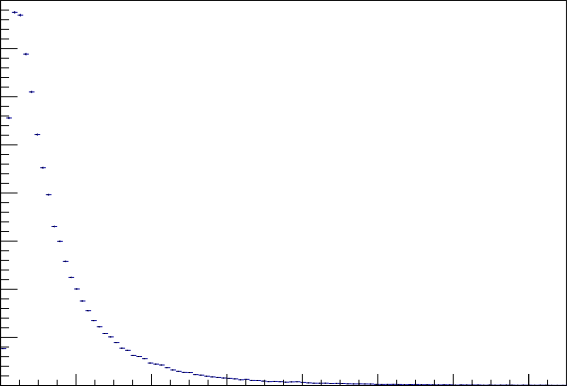
\includegraphics[width=0.8\textwidth]{detector/lab0_FD_OWNPV}};
        \begin{scope}[x={(image.south east)},y={(image.north west)}]
            \foreach \x in {0, ..., 7}
            {
                \tikzmath{\xpos = (\x / 7) * 0.934; \xtext = 20 * \x;}
                \node at (\xpos, -0.027) {\pgfmathprintnumber[fixed,precision=0,fixed zerofill=true]{\xtext}};
            }
            \foreach \y/\ytext in {0, ..., 8}
            {
                \tikzmath{\ypos = (\y / 8); \ytext = 10 * \y;}
                \node[anchor=east] at (0.005, \ypos) {\pgfmathprintnumber[fixed,precision=0,fixed zerofill=true]{\ytext}};
            }
            \node[anchor=south] at (0.03, 1.) {\({\times \num{e3}}\)};
            \node[anchor=east] at (1.0, -0.10) {\Bs~flight distance~[\si{\mm}]};
        \end{scope}
    \end{tikzpicture}
    \caption{
        Flight distance distribution of the \Bs~candidates from simulated \BsDsPi~decays.
        The exponential decrease corresponds with the decay of particles. The steep turn-on for small distances is caused by the acceptance of the \lhcb~trigger.}
    \label{fig:detector_FD}
\end{figure}

\subsection{Calorimetry}
\label{sec:calorimetry}

Downstream of the tracking detectors two calorimeters are located: an electromagnetic calorimeter~(\ecal) and a hadronic calorimeter (\hcal)~\cite{Perret:2015pla}.
The calorimeters are designed to stop most incoming particles and provide a measurement of their energy.
The \ecal detects electrons and photons, using an array of scintillating material of about \num{25}~radiation lengths to produce an electromagnetic shower response.
A single layer of scintillating pads~(\spd) is situated directly upstream of the~\ecal.
The pads track charged particles, and can therefore aid in distinguishing between electron and photon clusters in the~\ecal.
Finally, a two radiation lengths thick preshower detector~(\presh) is located directly upstream of the~\ecal, distinguishing electrons and photons from hadrons, as the latter are less likely to produce a contained shower.

The~\hcal has a thickness of \num{5.6}~radiation lengths.
It uses iron as absorber and scintillating tiles as active material.
It is designed to absorb all hadrons, allowing only muons to traverse into the downstream muon detectors.

\subsection{Particle identification}
\label{sec:det_pid}

Particle identification is obtained by a combination of the two Ring-Imaging~Cherenkov (\rich)~subdetectors, as well as the calorimeters and the muon stations.
The \rich{}es~\cite{LHCb-DP-2012-003} each consist of a container of active medium of different refractive index, which the produced particles traverse.
Whenever the speed of these particles exceeds the speed of light in one of these media, a cone-shaped burst of photonic Cherenkov radiation is emitted.
These photons are reflected in a set of mirrors mounted outside the fiducial volume of the container, and are subsequently picked up by arrays of photomultiplier tubes~(PMTs).
The diameter of a Cherenkov cone is a measure of the speed of the particle, which, together with its momentum as determined from the tracking detectors, allows determination of the particle's mass.
The \rich{}es are mostly used to discriminate between the various types of hadrons produced in the \({\proton\proton}\)~collisions: pions, kaons, and protons.
The active media used in~\rich1 and~\rich2 are~\cfourften, best suited for tracks with momenta up to~\SI{10}{\GeVc}, and~\cffour, for tracks with higher momenta up to~\SI{60}{\GeVc}, respectively.

To identify the other types of particles produced in the collisions, muons and electrons\footnote{The neutral particles that are also produced, \eg~photons, \piz~mesons, and neutrons, are not used by any of the analyses presented in this thesis, and therefore omitted from the discussion.}, the electromagnetic calorimeter and the muon stations are used.
Electrons are stopped by the electromagnetic calorimeter, and identified by their energy deposit.
Muons are the only particles traversing both the~\ecal and the~\hcal, and are identified by their tracks in the four muon stations located downstream of the calorimeters.

The data yielded by the~\rich{}es is analysed to yield quantitative information on the likelihood of a track belonging to a particle of a particular species.
The information of all RICH~PMTs from a single event is analysed simultaneously.
The algorithm starts by assuming the pion hypothesis for each track and computing the total likelihood under that assumption.
It then iteratively changes the hypothesis of each track if doing so improves the likelihood, until the maximum likelihood is reached.
The parameter of interest is then the difference in log-likelihood~(DLL) between two hypotheses.
For example, \dllkpi~represents the discrimination between the kaon and pion hypothesis of a track: a high value means the kaon hypothesis is more likely, while a low value tends towards the pion hypothesis.
\Cref{fig:detector_PID} demonstrates the necessity of using this information.

\begin{figure}[htb] \centerfloat
    \begin{tikzpicture}
        \node[anchor=south west,inner sep=0] (image) at (0,0) {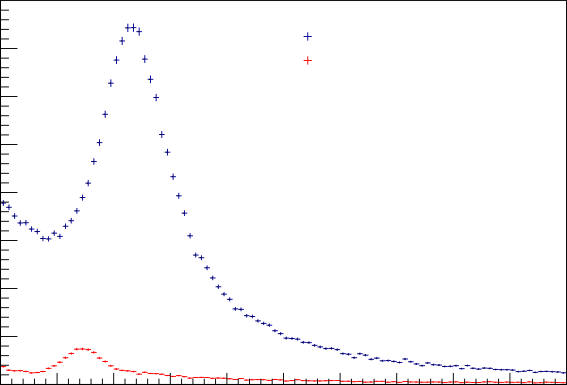
\includegraphics[width=0.8\textwidth]{detector/lab0_MM}};
        \begin{scope}[x={(image.south east)},y={(image.north west)}]
            \foreach \x in {0, ..., 10}
            {
                \tikzmath{\xpos = (\x / 10); \xtext = 50 * \x + 5300;}
                \node at (\xpos, -0.027) {\pgfmathprintnumber[fixed,precision=0,fixed zerofill=true,1000 sep={}]{\xtext}};
            }
            \foreach \y/\ytext in {1, ..., 8}
            {
                \tikzmath{\ypos = (\y / 8); \ytext = 1000 * \y;}
                \node[anchor=east] at (0.005, \ypos) {\pgfmathprintnumber[fixed,precision=0,fixed zerofill=true,1000 sep={}]{\ytext}};
            }
            % Legend
            {
                \node[anchor=base west] at (0.55, 0.890) {All data};
                \node[anchor=base west] at (0.55, 0.827) {With PID~selection};
            }
            \draw[gray,dashed] (.1338, 0.004) -- (.1338, 0.996) node [at end,below,rotate=90,anchor=south east,inner ysep=.5ex] {\tiny \Bs~mass};
            \node[anchor=east] at (1.0, -0.10) {\DsmpKpm~invariant mass~[\si{\MeVcc}]};
        \end{scope}
    \end{tikzpicture}
    \caption{
        The \DsmpKpm, \DsmpKKPi~invariant mass distribution of the full data set corresponding to an integrated luminosity of~\SI[mode=text]{3}{\per\femto\barn}, after the selection presented in \cref{sec:BsDsK_TD_Selection}, with and without PID selection on the companion track.
        The large peak in the distribution without the selection comes from misidentified \BsDsPi~decays, with a shifted mass due to the wrong mass hypothesis assigned to the companion track.
        The \BsDsK~mass peak (around~\SI{5367}{\MeVcc}) only becomes visible after a requirement on the \dllkpi~of the companion track.}
    \label{fig:detector_PID}
\end{figure}

\clearpage
\subsection{Trigger}
\label{sec:trigger}

The rate at which \({\proton\proton}\)~collisions take place in the detector is far greater than can conceivably be stored on disk.
In order to bring down the rate to a manageable level, a three-stage trigger~\cite{LHCb-DP-2012-004} selects only relevant events to be stored.
The first stage is a hardware trigger, called the Level~0 (\lzero)~trigger, which searches for tracks and clusters with high transverse momentum~(\pt) in the muon and calorimeter systems.
This stage brings the event rate down from \SI{40}{\MHz}~of collisions to an output rate of~\SI{1}{\MHz}.
The following two stages are both software-based, and these high-level triggers are called~\hltone and~\hlttwo.
They further reduce the event rate to a few~\si{\kHz}, which is low enough to allow storage on disk.
For the analyses presented in this thesis, the high-level triggers use a multivariate algorithm~\cite{Gligorov:2012qt} to require a vertex, displaced from the \({\proton\proton}\)~interaction point, consistent with the signature of a \bquark-meson decay (as illustrated in \cref{fig:detector_topology}).

\begin{figure}[htb] \centerfloat
    \begin{tikzpicture}
        \node[anchor=south west,inner sep=0] (image) at (0,0) {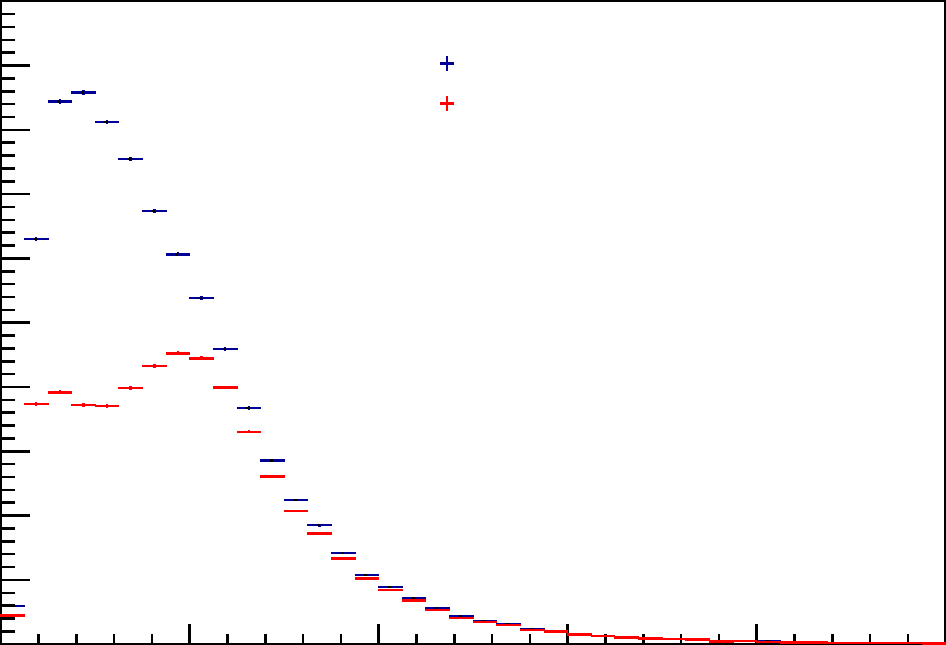
\includegraphics[width=0.8\textwidth]{detector/lab1_PT}};
        \begin{scope}[x={(image.south east)},y={(image.north west)}]
            \foreach \x in {0, ..., 5}
            {
                \tikzmath{\xpos = (\x / 5); \xtext = 5 * \x;}
                \node at (\xpos, -0.027) {\pgfmathprintnumber[fixed,precision=0,fixed zerofill=true,1000 sep={}]{\xtext}};
            }
            \foreach \y/\ytext in {0, ..., 10}
            {
                \tikzmath{\ypos = (\y / 10); \ytext = 10 * \y;}
                \node[anchor=east] at (0.005, \ypos) {\pgfmathprintnumber[fixed,precision=0,fixed zerofill=true,1000 sep={}]{\ytext}};
            }
            \node[anchor=south] at (0.03, 1.) {\({\times \num{e3}}\)};
            % Legend
            {
                \node[anchor=base west] at (0.480, 0.890) {All data};
                \node[anchor=base west] at (0.480, 0.827) {\lzero~triggered by companion};
            }
            \node[anchor=east] at (1.0, -0.10) {Companion~\pt~[\si{\GeVc}]};
        \end{scope}
    \end{tikzpicture}
    \caption{
        Transverse momentum distribution of companion \pipm~candidates from simulated \BsDsPi~decays, with and without the requirement that \lzero~triggered on the calorimeter cluster induced by that pion.
        It can be seen that for high-transverse momentum tracks, the \lzero~trigger usually triggered on those tracks, while for low-\pt~tracks it usually fired on another object in the event.}
    \label{fig:detector_companion_PT}
\end{figure}

\clearpage
\section{Simulation}
\label{sec:simulation}

In the analyses presented in this thesis, simulated samples are used to determine the selection efficiency of certain decays, as well as parameterise mass distributions of both signal and background channels.

The \proton\proton~collisions are generated using \pythia~\cite{Sjostrand:2007gs,Sjostrand:2006za} with a specific \lhcb configuration~\cite{LHCb-PROC-2010-056}.
Decays of hadronic particles are described by \evtgen~\cite{Lange:2001uf}, in which final-state radiation is generated using \photos~\cite{Golonka:2005pn}.
The interaction of the generated particles with the detector, and its response, are implemented using the \geant toolkit~\cite{Allison:2006ve,Agostinelli:2002hh} as described in Ref.~\cite{LHCb-PROC-2011-006}.
A software emulation of the \lzero~trigger is run on this response.
The next steps are the same as for data: \hltone, \hlttwo, and the reconstruction are applied, such that the simulated samples match the data as closely as possible.

